% Chapter 1 begins here
\Chapter{INTRODUCTION}
	\Section{Test} 
	\label{sec:int}
	
	This is explained in Section \ref{sec:int}. Now you will see a listing example:
	% An example for enumerate
	\begin{enumerate}
	  \item Suppression of hepatic glucose production
	  \item Stimulation of hepatic glucose uptake
	  \item Stimulation of glucose uptake by peripheral tissues,
	  mainly muscle
	\end{enumerate}
	
	\begin{quotation}
	This is a quotation. \cite{HK}
	\end{quotation}
	
	
	\Subsection{Test}
	
	Table format:
	\begin{table}[ht]
		\caption{Nonlinear Model Results}   % title of Table
		\centering                          % used for centering table
		\begin{tabular}{c c c c}            % centered columns (4 columns)
		\hline\hline                        % inserts double horizontal lines
		Case & Method\#1 & Method\#2 & Method\#3 \\ [0.5ex] % inserts table heading
		\hline                              % inserts single horizontal line below heading
		1 & 50 & 837 & 970  \\              % inserting the body of the table
		2 & 47 & 877 & 230  \\
		3 & 31 & 25  & 415  \\
		4 & 35 & 144 & 2356 \\
		5 & 45 & 300 & 556 \\ [1ex]         % [1ex] adds vertical space
		\hline                              % inserts single line
		\end{tabular}
		\label{table:nonlin}                % is used to refer this table in the text
	\end{table}

	Figure format:
	\begin{figure}[ht]
	  \centering                % centering figure
	  \scalebox{0.5}            % rescale the figure by a factor of 0.8
	  {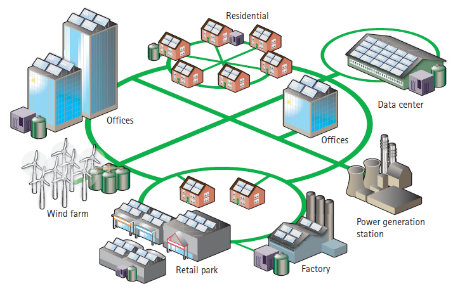
\includegraphics{microgrid.png}}   % importing figure
	  \caption{Fuel Metabolism results with Method A}        % title of figure
	  \label{fig:exm}                  % labelling to refer it inside the text
	\end{figure}
	
	\Section{Microgrid Structure}
	(Empty, Mg has distributed micro-sources, distributed consumers, distributed storage, common sources, common storages, and centralized control)\cite{wood2012power}
	
	Other format of citing some web link\cite{bworld}.
	
	\Section{Modeling Description}
	A microgrid is a localized grouping of electricity sources and loads that normally operates connected to and synchronous with the traditional centralized grid (macrogrid), but can disconnect and function autonomously as physical and/or economic conditions dictate\footnote{About Microgrid: \url{http://building-microgrid.lbl.gov/about-microgrids}}.
	
	Microgrids are modern, small-scale versions of the centralized electricity system. They achieve specific local goals, such as reliability, carbon emission reduction, diversification of energy sources, and cost reduction, established by the community being served. Like the bulk power grid, smart microgrids generate, distribute, and regulate the flow of electricity to consumers, but do so locally. Smart microgrids are an ideal way to integrate renewable resources on the community level and allow for customer participation in the electricity enterprise\footnote{What are smart microgrid? \url{http://galvinpower.org/microgrids}}. 
	In this model we want to achieve three goals:
	\begin{itemize}
	\item An ingenious scheduler of power energy in Microgrid, such as managing battery reservation and renewable energy generation. 
	\item Minimize the cost of Microgrid in the perspective of customer in such Microgrid. Also we should meet the requirement of such system in a reliable, efficient, and sustainable condition.
	\item Try to find out a proper way to simulate the energy demand such that we can maintain microgrid in a economic performance. 
	\end{itemize}
	
	\clearpage
	